

\section{Introduction}
The range of bacterial growth rates can be enormous. In natural environments,
doublings occur approximately once per year whereas in comfortable laboratory
conditions, growth can be rapid with several divisions per hour.
This remarkable diversity illustrates the intimate relationship between
environmental conditions and the rates at which cells convert nutrients into
new cellular material. This relationship between the environment and cellular
growth rate has remained a major topic of inquiry in bacterial physiology for
over a century \citep{jun2018}. In 1958, Schaecter, Mall\o e, and Kjeldgaard
reported the discovery of a strong, linear relationship between the total
cellular protein content and growth rate,  revealing a fundamental relationship
between the environment and the composition of the intracellular milieu \citep{schaechter1958}.
Over the past decade, a remarkable body
of work has examined this relationship with single-protein resolution using
modern methods of mass spectrometry \citep{valgepea2013,
peebo2015, schmidt2016} and ribosomal profiling \citep{li2014} which permit a
quantitative investigation of the relationship between gene expression and
growth rate. This body of experimental data places us in the auspicious position to
explore how the abundance of fundamental protein complexes are related to the
growth rate of the population and interrogate what biological processes may set
the speed limit of bacterial growth.

In this work, we seek to leverage a collection of proteomic data sets of
\textit{Escherichia coli} across 31 growth conditions to
quantitatively explore what biological processes may set the speed limit of
bacterial growth. Broadly speaking, we entertain three classes of hypotheses
illustrated in \FIG{categories}. First, we consider potential limits on the
transport of nutrients into the cell. We address this hypothesis by performing
an order-of-magnitude estimate for how many carbon atoms would be needed to
build a cell and consider how many transporters may be needed to facilitate this
requirement given a 6000 second division time.  As a second hypothesis, we consider there exists a fundamental limit on how
quickly the cell can generate ATP. We approach this hypothesis from two angles,
considering how many ATP synthase complexes must be needed to churn out enough
ATP to power protein translation followed by an estimation of how many electron
transport complexes must be present to maintain the proton motive force. Our third and final class of hypotheses centers on the synthesis of a variety of
biomolecules. Our focus is primarily on the stages of the central dogma as we
estimate the number of protein complexes needed for DNA replication,
transcription, and protein translation.

With estimates in hand for each of these processes, we turn to our collection
of data sets to assess the accuracy of our estimates. In broad terms, we find
that the majority of our estimates are exceeded by the experimental
observations, allowing us to systematically scratch off the hypotheses
diagrammed in \FIG{categories} as setting the speed limit. Ultimately, we
find that protein translation (particularly the generation of new ribosomes)
acts as the rate limiting step of bacterial division. We again leverage the
quantitative nature of this data set and present a quantitative model of the
relationship between the fraction of the proteome devoted to ribosomes and the
speed limit of translation, revealing a fundamental tradeoff between the
translation capacity of the ribosome pool and the maximal cellular growth rate.

\begin{figure}
    \centering{
    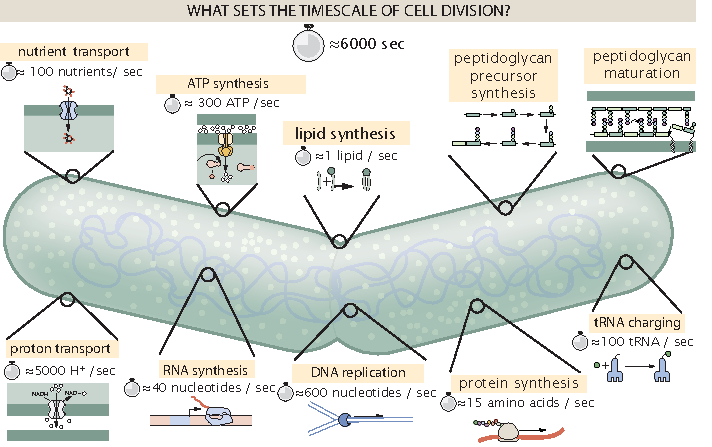
\includegraphics{main_figs/schematic_categories.pdf}
    \caption{\textbf{Transport and synthesis processes necessary for cell division.} 
            We consider an array of processes necessary for a cell to double its
            molecular components. Such processes include the transport of carbon
            across the cell membrane, the production of ATP, and fundamental
            processes of the central dogma namely RNA, DNA, and protein
            synthesis. A schematic of each synthetic or transport category is
            shown with an estimate of the rate per macromolecular complex. In
            this work, we consider a standard bacterial division time of
            $\approx$ 6000 sec.}
    \label{fig:categories}
    }
\end{figure}


